%%%%%%%%%%%%%%%%%%%%%%%%%%%%%%%%%%%%%%%%%%%%%%%%%%%%%%%%%%%%%%%%%%%%%%%%%%%

\chapter{Number Theory}


%%%%%%%%%%%%%%%%%%%%%%%%%%%%%%%%%%%%%%%%%%%%%%%%%%%%%%%%%%%%%%%%%%%%%%%%%%%

\section{Integers}

An \emph{integer} is a whole number. It can be positive, negative, or
zero. Examples of integers include $-13$, $-1$, $0$, and $42$. When we
talk about all the whole numbers, we can use the name \emph{integer}
to refer to them, or we can list all the whole numbers like so:
\[
\dots, -4, -3, -2, -1, 0, 1, 2, 3, 4, \dots
\]
But for convenience, we usually write $\ZZ$ to denote the set of all
integers:
\[
\ZZ
=
\{\dots, -3, -2, -1, 0, 1, 2, 3, \dots\}.
\]
In Sage, the set of all integers is represented as \verb!ZZ! and a
single integer is represented using \verb!Integer!:
%
\begin{lstlisting}
sage: ZZ
Integer Ring
sage: type(ZZ)
<type 'sage.rings.integer_ring.IntegerRing_class'>
sage: 1 in ZZ
True
sage: -1 in ZZ
True
sage: 3.1415 in ZZ
False
sage: type(3)
<type 'sage.rings.integer.Integer'>
sage: Integer
<type 'sage.rings.integer.Integer'>
\end{lstlisting}
%
Notice that in the above code listing, we used \verb!in! to test
whether or not a number is an integer. The command
%
\begin{lstlisting}
sage: 1 in ZZ
True
\end{lstlisting}
%
gives the result \verb!True! because $1$ is an integer. On the other
hand, the command
%
\begin{lstlisting}
sage: 3.1415 in ZZ
False
\end{lstlisting}
%
gives \verb!False! because $3.1415$ is not an integer.


%%%%%%%%%%%%%%%%%%%%%%%%%%%%%%%%%%%%%%%%%%%%%%%%%%%%%%%%%%%%%%%%%%%%%%%%%%%

\section{Prime numbers}

A positive integer $n > 1$ is a \emph{prime} number if its factors are
exclusively $1$ and itself. The integer $2$ is prime because its only
factors are $1$ and $2$. As a matter of fact, $2$ is the smallest
prime integer. The next prime after $2$ is $3$. However, the next
integer $4$ is not prime because $2$ is a factor of $4$. In Sage, the
command \verb!is_prime! tests whether or not an integer is prime. We
can obtain the first $15$ prime numbers using the command
\verb!primes_first_n!.

\begin{lstlisting}
sage: is_prime(1)
False
sage: is_prime(2)
True
sage: is_prime(3)
True
sage: is_prime(4)
False
sage: primes_first_n(15)
[2, 3, 5, 7, 11, 13, 17, 19, 23, 29, 31, 37, 41, 43, 47]
\end{lstlisting}

If $n$ is an integer, the command \verb!next_prime! can be used to
compute the next prime integer starting from $n$. Likewise, the command
\verb!previous_prime! computes the previous prime integer starting
from $n$.
%
\begin{lstlisting}
sage: next_prime(-25)
2
sage: next_prime(1)
2
sage: next_prime(50)
53
sage: previous_prime(50)
47
sage: previous_prime(3)
2
sage: previous_prime(2)
Traceback (most recent call last):
...
ValueError: no previous prime
\end{lstlisting}
%
The command
%
\begin{lstlisting}
sage: next_prime(-25)
2
\end{lstlisting}
%
results in \verb!2! because $2$ is the smallest prime. In other words,
there are no primes smaller than $2$, which explains the result of the
following command:
%
\begin{lstlisting}
sage: previous_prime(2)
Traceback (most recent call last):
...
ValueError: no previous prime
\end{lstlisting}

There are various questions we can ask about prime numbers. For
example, how many prime integers are there? Over two thousand years
ago, the Greek mathematician Euclid proved that there are infinitely
many primes. No matter how high up we count, there is still a prime
number to be found.

Here's another question: If $n$ is a positive integer greater than
$1$, how many primes are there between $1$ and $n$? In the case of $n
= 50$, we could use the command \verb!primes_first_n! to list the
first 20 primes, then count how many of those primes are less than or
equal to $50$.
%
\begin{lstlisting}
sage: primes_first_n(20)
[2, 3, 5, 7, 11, 13, 17, 19, 23, 29, 31, 37, 41, 43, 47, 53, 59, 61, 67, 71]
sage: P = [2, 3, 5, 7, 11, 13, 17, 19, 23, 29, 31, 37, 41, 43, 47]; P
[2, 3, 5, 7, 11, 13, 17, 19, 23, 29, 31, 37, 41, 43, 47]
sage: len(P)
15
\end{lstlisting}
%
In the above code listing, we put all the primes less than or equal to
$50$ into the list \verb!P!. We then used the command \verb!len! to
obtain the length of that list. From the above output, there are $15$
primes less than or equal to $n = 50$.

Alternatively, we can let the command \verb!prime_pi! do all the hard
work for us. Given an integer $n$---either positive, negative, or
zero---the command \verb!prime_pi(n)! counts how many primes are less
than or equal to $n$.
%
\begin{lstlisting}
sage: prime_pi(50)
15
sage: prime_pi(100)
25
sage: prime_pi(1000)
168
sage: prime_pi(10000)
1229
sage: prime_pi(0)
0
sage: prime_pi(-10)
0
\end{lstlisting}
%
To study the output of \verb!prime_pi(n)! as the integer \verb!n!
increases, we could substitute $n = 1, 2, 3, \dots$ into the
command. Or we could use \verb!plot! together with \verb!prime_pi! to
visualize how the output of \verb!prime_pi! changes as $n$ increases
in value. Figure~\ref{fig:number_theory:prime_pi_for_n_leq_100}
illustrates the change in the values of \verb!prime_pi! as $n$ takes
on all integer values from $0$ up to and including $100$. Notice that
when $n = 50$, the output of \verb!prime_pi! is $15$, which confirms
our computation above. The horizontal axis shows integer values of $n$
from $0$ to $100$, inclusive, while the vertical axis shows the output
of the command \verb!prime_pi(n)!. The figure was produced using the
following code listing:
%
\begin{lstlisting}
sage: P = plot(prime_pi, 0, 100)
sage: V = line([(50,0), (50,25)], color="red")     # vertical line
sage: H = plot(15, xmin=0, xmax=100, color="red")  # horizontal line
sage: P + H + V
\end{lstlisting}
%
\begin{figure}[!htbp]
\centering
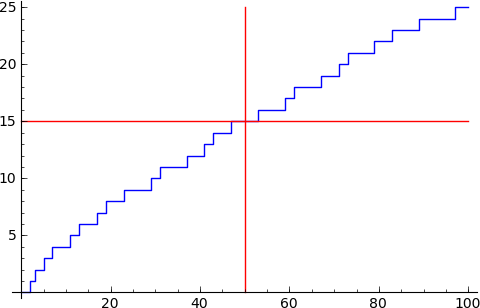
\includegraphics[scale=0.8]{images/prime-pi-100}
\caption{Values of \texttt{prime\_pi(n)} for $n = 0, 1, 2, \dots, 100$.}
\label{fig:number_theory:prime_pi_for_n_leq_100}
\end{figure}
%
And Figure~\ref{fig:number_theory:prime_pi_for_n_leq_1000} shows the
behavior of \verb!prime_pi! as $n$ increases from $0$ to $1000$. The
figure was produced using the command:
%
\begin{lstlisting}
sage: plot(prime_pi, 0, 1000)
\end{lstlisting}
%
\begin{figure}[!htbp]
\centering
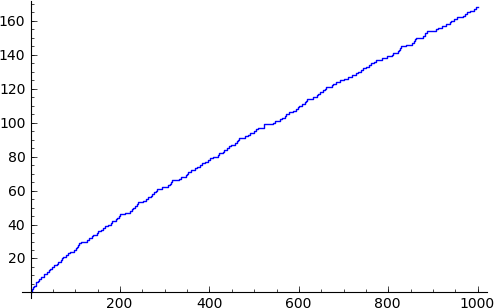
\includegraphics[scale=0.8]{images/prime-pi-1000}
\caption{Values of \texttt{prime\_pi(n)} for $n = 0, 1, 2, \dots, 1000$.}
\label{fig:number_theory:prime_pi_for_n_leq_1000}
\end{figure}


%%%%%%%%%%%%%%%%%%%%%%%%%%%%%%%%%%%%%%%%%%%%%%%%%%%%%%%%%%%%%%%%%%%%%%%%%%%

\section{Divisibility}

For any two integers $a$ and $n$, we say that $a$ \emph{divides} $n$
if $a$ is a factor of $n$. That is, if we can find an integer $b$ such
that $n = ab$, then $a$ is a factor of $n$. In that case, $b$ is also
a factor of $n$. The integer $2$ divides, or is a factor of, $4$
because $4 = 2 \times 2$. Similarly, both $2$ and $3$ are factors of,
or both divide, $6$ because $6 = 2 \times 3$.

Does every positive integer have a factor? Yes. In fact, if $n > 1$ is
an integer, then $n$ has a factor that is greater than $1$. We can
make a stronger claim: Every integer $n > 1$ has a prime factor. A
factorization, or prime factorization, of $n$ is product containing
all the primes that divide $n$. Examples of prime factorizations
include $4 = 2 \times 2$ and $6 = 2 \times 3$. However, $8 = 2 \times 4$
is not a prime factorization of $8$ because the product $2 \times 4$
has $4$, which is not prime.

To find all the positive divisors of an integer, use the command
\verb!divisors!.
%
\begin{lstlisting}
sage: divisors(4)
[1, 2, 4]
sage: divisors(6)
[1, 2, 3, 6]
sage: divisors(8)
[1, 2, 4, 8]
\end{lstlisting}
%
To write $n$ as a product of primes, use \verb!factor!.

\begin{lstlisting}
sage: factor(4)
2^2
sage: factor(6)
2 * 3
sage: factor(8)
2^3
\end{lstlisting}
